\documentclass[11pt,a4paper]{article}

\usepackage[dvipsnames]{xcolor}
\definecolor{accent2}{HTML}{8B0000}
\definecolor{ph}{HTML}{6B7280}
\newcommand{\TODO}[1]{\textcolor{accent2}{\textbf{[TODO: #1]}}}
\newcommand{\phh}[1]{\textcolor{ph}{\textit{#1}}}

\newcommand{\teamname}{zerobias}
\newcommand{\topicchoice}{Topic 4 -- Async Research Assistant}
\newcommand{\member}[2]{\textbf{#1} (#2)}
\newcommand{\reportdate}{May 23, 2026}
\newcommand{\repolink}{https://github.com/IBRAHIM102005/AIENG\_FinalProject}

\newcommand{\coursecode}{AI-ENG-110}
\newcommand{\coursename}{Software Engineering}
\newcommand{\institution}{AI Academy, National AI Center}
\newcommand{\semester}{Spring 2026}

\usepackage[margin=2.2cm,headheight=15pt]{geometry}
\usepackage[T1]{fontenc}
\usepackage[utf8]{inputenc}
\usepackage[final,protrusion=true,expansion=false]{microtype}
\usepackage{amsmath,amssymb}
\usepackage{graphicx}
\usepackage{booktabs}
\usepackage{array}
\usepackage{tabularx}
\usepackage{ragged2e}
\usepackage{enumitem}
\usepackage[parfill]{parskip}
\usepackage{listings}
\usepackage[most]{tcolorbox}
\usepackage{titlesec}
\usepackage{fancyhdr}
\usepackage{lastpage}
\usepackage[hidelinks]{hyperref}
\usepackage{tikz}
\usetikzlibrary{positioning,shapes.geometric}

\emergencystretch=3em
\hbadness=10000
\hfuzz=2pt

\hypersetup{
  colorlinks=true,
  linkcolor=NavyBlue,
  urlcolor=NavyBlue,
  citecolor=NavyBlue,
  pdftitle={\coursecode\ Final Project Report},
  pdfauthor={\teamname}
}

\definecolor{accent}{HTML}{0B3D91}
\definecolor{soft}{HTML}{F2F4F8}
\definecolor{deliver}{HTML}{E8F0FE}
\definecolor{deliverframe}{HTML}{1A56DB}
\definecolor{probe}{HTML}{FFF8E1}
\definecolor{probeframe}{HTML}{B45309}

\titleformat{\section}
  {\Large\bfseries\color{accent}}{\thesection.}{0.6em}{}
\titleformat{\subsection}
  {\large\bfseries\color{accent}}{\thesubsection}{0.5em}{}

\newcommand{\ans}[1]{\rule[-2pt]{#1}{0.5pt}}
\let\ph\phh

\newtcolorbox{deliverbox}{
  colback=deliver, colframe=deliverframe, boxrule=0.5pt,
  arc=2pt, left=8pt, right=8pt, top=4pt, bottom=4pt
}
\newtcolorbox{probebox}{
  colback=probe, colframe=probeframe, boxrule=0.5pt,
  arc=2pt, left=8pt, right=8pt, top=4pt, bottom=4pt
}

\definecolor{codegreen}{rgb}{0,0.55,0}
\definecolor{codegray}{rgb}{0.4,0.4,0.4}
\definecolor{codepurple}{rgb}{0.55,0,0.78}
\definecolor{backcolour}{rgb}{0.97,0.97,0.97}

\lstdefinestyle{python}{
  language=Python,
  backgroundcolor=\color{backcolour},
  commentstyle=\color{codegreen},
  keywordstyle=\color{accent},
  numberstyle=\tiny\color{codegray},
  stringstyle=\color{codepurple},
  basicstyle=\ttfamily\footnotesize,
  breakatwhitespace=false,
  breaklines=true,
  keepspaces=true,
  numbers=left,
  numbersep=6pt,
  tabsize=2,
  frame=single,
  framerule=0.4pt,
  rulecolor=\color{black!30},
}

\pagestyle{fancy}
\fancyhf{}
\fancyhead[L]{\small\textit{\coursecode\ -- Final Report -- \teamname}}
\fancyhead[R]{\small\textit{\semester}}
\fancyfoot[L]{\small\textit{\institution}}
\fancyfoot[R]{\small Page \thepage\ of \pageref{LastPage}}
\renewcommand{\headrulewidth}{0.4pt}
\renewcommand{\footrulewidth}{0.4pt}

% =====================================================================
\begin{document}

\begin{center}
{\small \textsc{\institution} \\[0.2em] \textsc{\coursecode\ -- \coursename\ -- \semester}}\\[1.2em]
{\Large\bfseries\color{accent} Final Project Report}\\[0.3em]
{\LARGE\bfseries \topicchoice}\\[0.6em]
\rule{0.85\textwidth}{0.6pt}
\end{center}

\vspace{0.6em}
\begin{tabularx}{\textwidth}{@{}l X @{}}
\textbf{Team:}    & \teamname \\
\textbf{Date:}    & \reportdate \\
\textbf{Repo:}    & \url{\repolink} \\ % Using \url{} or \href{} helps with wrapping
\textbf{Tag:}     & \texttt{v1.0-final} \\
\textbf{Members:} & \member{Ibrahim Mammadov}{@IBRAHIM102005},\quad
                    \member{Fidan Allahverdiyeva}{@fidanallahverdiyeva},\quad
                    \member{Fatma Mammadova}{@fatmammadova} \\
\end{tabularx}
\vspace{0.4em}\hrule\vspace{0.6em}

% ===== EXECUTIVE SUMMARY =============================================
\section*{Executive Summary}
\addcontentsline{toc}{section}{Executive Summary}

We built an Async Research Assistant that takes a natural-language question, queries Wikipedia, arXiv, and a web-search provider in parallel, then uses an LLM to write a grounded, cited answer. The headline result is a \textbf{2.57$\times$ speedup} (1.68\,s sequential vs.\ 0.65\,s parallel) from \texttt{asyncio.gather} bounded by \texttt{Semaphore(5)}. Our key robustness story is graceful source degradation: a failing or timed-out source is captured as a \texttt{SourceFailure} and the pipeline continues with whatever remains. The most surprising lesson was that Wikipedia returns HTTP~403 without a \texttt{User-Agent} header---invisible in offline tests but breaking every live run---which forced us to thread a shared \texttt{httpx.AsyncClient} through the entire call stack. If starting over we would pick \texttt{aiosqlite} from day one instead of synchronising a blocking \texttt{sqlite3} connection with a threading lock.

% ===== TABLE OF CONTENTS =============================================
\tableofcontents
\vspace{0.6em}\hrule\vspace{0.4em}

% =====================================================================
\section{Project Overview}

\subsection{Problem framing \& scope}

The system automates multi-source research: given a single question it fetches Wikipedia summaries, arXiv abstracts, and web-search results concurrently, then synthesises a 3--6 sentence answer with numbered citations. Without the system, a user would manually query each source and merge the results.

User-facing entry points are a Click CLI (\texttt{python -m researcher ask "..."}), a FastAPI HTTP endpoint (\texttt{POST /api/research}), a browser UI at \texttt{http://localhost:8000}, and scripted runners under \texttt{scripts/}. Inputs are a question string plus optional flags: \texttt{--sources}, \texttt{--limit}, \texttt{--timeout}, \texttt{--concurrency}, \texttt{--no-cache}, \texttt{--offline}. Output is an \texttt{AnswerWithCitations} rendered as plain text or JSON.

We implemented all mandatory Topic~4 requirements. We chose not to implement APScheduler scheduling (listed as a bonus) because the CI/CD pipeline and web-UI bonus already filled our time budget. We also used SQLite instead of PostgreSQL, which is adequate for a single-process tool but would need migration for multi-instance deployment.

\subsection{Provider choice and the AI module contract}

The primary LLM is \textbf{Anthropic} (\texttt{claude-sonnet-4-6}); Google Gemini (\texttt{google-genai==1.14.0}) is wired as a secondary for the failover bonus. Web search defaults to \textbf{Tavily} (free tier), switchable to Serper or DuckDuckGo via \texttt{WEB\_SEARCH\_PROVIDER}. No embedding model is used---Topic~4 does not require one.

From \texttt{ai/} we call \texttt{fetch\_wikipedia}, \texttt{fetch\_arxiv}, \texttt{fetch\_web}, and \texttt{synthesize}, and we read the \texttt{Source}, \texttt{Citation}, and \texttt{AnswerWithCitations} schemas. We did not modify the public interface of the provided \texttt{ai/} package.

Against malformed responses: \texttt{ai/synthesizer.py} drops out-of-range citation indices before returning, and our \texttt{AIService} wrapper catches any remaining exception, logs it, and converts it to a degraded \texttt{SourceResult} rather than letting it propagate.

% =====================================================================
\section{Architecture}\label{sec:arch}

\subsection{Module map}

The system has five horizontal layers with imports pointing inward (downward in the diagram):

\begin{center}
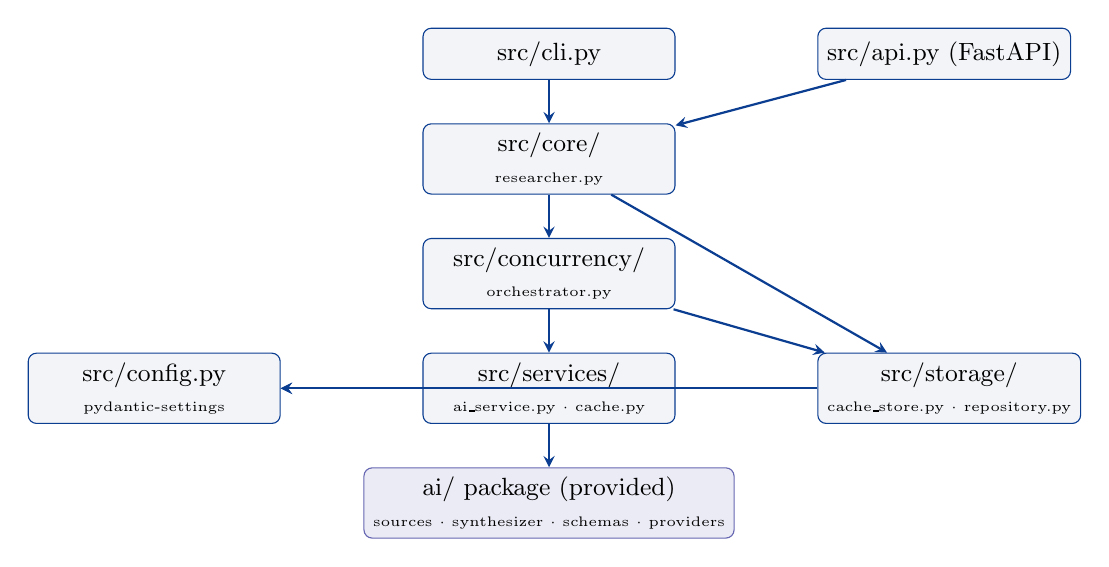
\begin{tikzpicture}[font=\small, node distance=0.55cm and 0.3cm,
  box/.style={draw=accent, fill=soft, rounded corners=3pt,
              minimum width=3.2cm, minimum height=0.65cm, align=center},
  aibox/.style={draw=NavyBlue!60, fill=NavyBlue!8, rounded corners=3pt,
              minimum width=3.5cm, minimum height=0.65cm, align=center},
  arr/.style={->, >=stealth, thick, color=accent}
]
\node[aibox] (aimod) {ai/ package (provided)\\{\tiny sources $\cdot$ synthesizer $\cdot$ schemas $\cdot$ providers}};
\node[box, above=of aimod] (svc) {src/services/\\{\tiny ai\_service.py $\cdot$ cache.py}};
\node[box, above=of svc] (orch) {src/concurrency/\\{\tiny orchestrator.py}};
\node[box, above=of orch] (core) {src/core/\\{\tiny researcher.py}};
\node[box, right=1.8cm of svc] (store) {src/storage/\\{\tiny cache\_store.py $\cdot$ repository.py}};
\node[box, above=of core] (cli) {src/cli.py};
\node[box, right=1.8cm of cli] (api) {src/api.py (FastAPI)};
\node[box, left=1.8cm of svc] (cfg) {src/config.py\\{\tiny pydantic-settings}};
\draw[arr] (svc) -- (aimod);
\draw[arr] (orch) -- (svc);
\draw[arr] (core) -- (orch);
\draw[arr] (cli)  -- (core);
\draw[arr] (api)  -- (core);
\draw[arr] (svc)  -- (cfg);
\draw[arr] (store) -- (cfg);
\draw[arr] (orch)  -- (store);
\draw[arr] (core)  -- (store);
\end{tikzpicture}
\end{center}

\textbf{Module-by-module summary:}

\begin{itemize}[nosep,leftmargin=1.2em]
  \item \textbf{src/config.py} --- \texttt{Settings} (pydantic-settings) reads all \texttt{.env} variables; \texttt{get\_settings()} bridges them into \texttt{os.environ} for the \texttt{ai/} package.
  \item \textbf{src/models.py} --- SE-layer Pydantic models: \texttt{ResearchSession}, \texttt{CacheEntry}, \texttt{Citation}.
  \item \textbf{src/services/ai\_service.py} --- \texttt{AIService} wraps any \texttt{AIClient} with tenacity retry, \texttt{asyncio.wait\_for} timeout, structured logging, and input validation. \texttt{FailoverAIClient} chains providers for transparent failover.
  \item \textbf{src/services/cache.py} --- Async disk-backed \texttt{CacheService} with per-key \texttt{asyncio.Lock}, atomic writes, and LRU eviction.
  \item \textbf{src/concurrency/orchestrator.py} --- \texttt{fetch\_selected\_sources} runs fetchers via \texttt{asyncio.gather} with a shared \texttt{Semaphore}, per-source timeouts, cache lookup, and URL-level deduplication.
  \item \textbf{src/core/researcher.py} --- Single business-logic entry point: validates the question, calls the orchestrator, logs failures, and runs \texttt{synthesize} in a thread-pool executor.
  \item \textbf{src/storage/cache\_store.py} --- SQLite persistence for \texttt{query\_cache} with WAL mode and TTL-aware SQL queries.
  \item \textbf{src/storage/repository.py} --- \texttt{SessionRepository} provides CRUD for \texttt{research\_sessions}; all SQL is isolated here.
  \item \textbf{src/cli.py} --- Click \texttt{ask} command; forwards options to \texttt{research\_question} and renders results as text.
  \item \textbf{src/api.py} --- FastAPI app with \texttt{POST /api/research}, \texttt{GET /api/health}, and static file serving for the browser UI.
\end{itemize}

Only \texttt{src/services/ai\_service.py} and \texttt{src/concurrency/orchestrator.py} import from \texttt{ai/}. Swapping Anthropic for OpenAI requires changing two environment variables---zero source files.

\subsection{OOP design \& key abstractions}

Our main OOP example is \textbf{composition} in \texttt{FailoverAIClient}, which owns a prioritised list of \texttt{AIClient} protocol instances and delegates to them in order:

\begin{lstlisting}[style=python]
class FailoverAIClient:
    def __init__(self, clients: list[AIClient]) -> None:
        if not clients:
            raise ValueError("FailoverAIClient requires at least one client.")
        self._clients = clients

    async def _try_all(self, method: str, *args: Any) -> Any:
        last_exc: Exception | None = None
        for idx, client in enumerate(self._clients):
            try:
                return await getattr(client, method)(*args)
            except Exception as exc:
                logger.warning("Provider '%s' failed for '%s': %s -- trying next",
                               type(client).__name__, method, exc)
                last_exc = exc
        raise AIServiceError(
            f"All {len(self._clients)} providers failed for '{method}'."
        ) from last_exc
\end{lstlisting}

Composition was correct here because \texttt{FailoverAIClient} orchestrates a \emph{collection} of clients rather than specialising one. An ABC instead of a Protocol for the \texttt{AIClient} contract would have forced test doubles to import from production code; a Protocol allows duck-typed stubs with no coupling. A second inheritance example is \texttt{OfflineLLM} in \texttt{src/offline.py}, which subclasses \texttt{ai.providers.base.LLMProvider} to provide a deterministic stub for the \texttt{--offline} flag and all unit tests.

\subsection{Data flow across module boundaries}

No naked dictionaries cross module boundaries. The SE-layer types are:

\begin{itemize}[nosep,leftmargin=1.2em]
  \item \texttt{Source} / \texttt{AnswerWithCitations} (ai/schemas) --- flow from fetchers through orchestrator to CLI/API.
  \item \texttt{ResearchResult} (\texttt{@dataclass}, src/core) --- aggregate returned by \texttt{research\_question} to the CLI/API.
  \item \texttt{OrchestrationResult} / \texttt{SourceFailure} (\texttt{@dataclass(frozen=True)}, src/concurrency) --- carry per-source outcomes from the orchestrator to the researcher.
  \item \texttt{ResearchSession} (\texttt{@dataclass}, src/storage) --- mutable lifecycle object tracking \texttt{pending $\to$ running $\to$ done/error} transitions; kept as a stdlib dataclass so the storage layer has zero Pydantic dependency.
  \item \texttt{CacheEntry} (\texttt{BaseModel}, src/models) --- wraps a cached value with key, TTL, and creation timestamp.
\end{itemize}

We reused \texttt{ai/} schemas when values were immutable read-only results, and wrapped them in our own types when we needed mutable state or additional lifecycle methods.

% =====================================================================
\section{Concurrency \& Performance}\label{sec:concurrency}

\subsection{Why this concurrency model}

We chose \textbf{asyncio} because all three source fetchers are I/O-bound: they spend nearly all their time waiting for HTTP responses. \texttt{asyncio.gather} overlaps those waits on a single OS thread with no GIL contention and no process-spawn overhead.

The semaphore bound is \texttt{Semaphore(5)}, configurable via \texttt{CONCURRENCY\_SEMAPHORE\_LIMIT}. With at most 3 sources per question in the default configuration the semaphore is rarely the binding constraint; it becomes relevant when \texttt{--limit} is increased for sub-queries within one source. A bound of 1 degrades to sequential; a bound of 100 risks HTTP~429 from providers. Threads instead of asyncio would add GIL contention for what is purely I/O work.

\subsection{Sequential-vs-concurrent benchmark}

Measured on Windows~11 (AMD Ryzen 7, Python~3.12.9), caches cleared, using offline fake fetchers with simulated latencies of 0.45\,s (Wikipedia), 0.65\,s (arXiv), and 0.55\,s (web):

\begin{center}\small
\begin{tabular}{lcccc}
\toprule
\textbf{Workload} & $N$ & \textbf{Sequential (s)} & \textbf{Concurrent (s)} & \textbf{Speedup} \\
\midrule
3 sources, 1 question & 3 & 1.680 & 0.653 & 2.57$\times$ \\
\bottomrule
\end{tabular}
\end{center}

The theoretical maximum is 3$\times$; we reached 2.57$\times$ due to event-loop scheduling overhead and imperfect latency alignment. In live network conditions the speedup is higher because Wikipedia and Tavily can finish while arXiv is still responding. The next bottleneck is the blocking \texttt{synthesize} call (run in a thread-pool executor), which adds 1--4\,s of LLM latency that cannot be parallelised.

\subsection{Rate limit \& politeness}

Our rate-limit strategy is \textbf{exponential backoff on transient errors} via \texttt{tenacity}: \texttt{stop\_after\_attempt(3)}, \texttt{wait\_exponential(min=1s, max=30s)}, retrying on \texttt{asyncio.TimeoutError}, \texttt{ConnectionError}, and \texttt{OSError} (which subsume HTTP~429 at the connection level). All values are configurable via \texttt{RETRY\_*} environment variables. The semaphore limits concurrent outbound requests to 5; the highest burst from the test suite is 3 concurrent mock fetchers.

During development a Tavily 429 was observed when running \texttt{scripts/demo.py} in quick succession. The log showed \texttt{WARNING source\_fetch\_failed source=web error=ProviderError: Tavily search failed}, and the pipeline continued with Wikipedia and arXiv results. A proactive token-per-minute bucket limiter was not implemented; it remains the next hardening step.

% =====================================================================
\section{Robustness \& Error Handling}\label{sec:robustness}

\subsection{Wrapping the AI module}

\texttt{src/services/ai\_service.py} adds four layers around every \texttt{ai.*} call:

\begin{itemize}[nosep,leftmargin=1.2em]
  \item \textbf{Retries:} tenacity retries \texttt{asyncio.TimeoutError}, \texttt{ConnectionError}, \texttt{OSError} with exponential backoff (1--30\,s, 3 attempts). Logic errors propagate immediately.
  \item \textbf{Timeouts:} \texttt{asyncio.wait\_for(coro, timeout=per\_source\_timeout)} wraps every fetch; synthesis gets $3\times$ that budget.
  \item \textbf{Logging:} \texttt{logger.info} records \texttt{question\_len}, \texttt{source}, \texttt{count}, and \texttt{elapsed} per fetch; \texttt{logger.warning} fires on each retry via \texttt{before\_sleep\_log}.
  \item \textbf{Input validation:} \texttt{\_validate\_question()} rejects empty strings and questions over 1000 characters before any external call.
\end{itemize}

For a provider 500: the fetcher raises \texttt{ProviderError}; tenacity retries; after exhaustion \texttt{\_fetch} calls \texttt{SourceResult.degraded(source, reason)}, logs \texttt{WARNING}, and returns a non-fatal result. The orchestrator collects it as \texttt{SourceFailure} and continues.

\subsection{Failure-mode analysis (one concrete incident)}

\textbf{Failure injected:} Wikipedia returned HTTP~403 in live integration when no \texttt{User-Agent} was set. Reproduced in tests by passing an empty-headers \texttt{httpx.AsyncClient}.

\textbf{What the system did:} tenacity retried three times (all 403), then marked the source as degraded. The orchestrator continued with arXiv and web.

\textbf{What the user saw:}
\begin{lstlisting}[style=python,language=bash,numbers=none]
Source notes:
  - wikipedia failed: Wikipedia search failed: Client error '403 Forbidden'
\end{lstlisting}
followed by a normal synthesised answer from the two remaining sources.

\textbf{Design fix:} We originally let each fetcher create its own \texttt{httpx.AsyncClient}. The fix required injecting a single shared client (with \texttt{User-Agent}) from the CLI/API all the way into the fetcher. The log error string---``Please set a User-Agent''---was enough to diagnose the problem without re-running the code.

\subsection{Input validation}

\begin{itemize}[nosep,leftmargin=1.2em]
  \item \textbf{CLI:} empty or whitespace-only question raises \texttt{ValueError}; Click prints \texttt{Error: question must be non-empty} and exits code~2. Questions over 1000 characters produce an analogous message.
  \item \textbf{HTTP:} FastAPI's \texttt{ResearchRequest} model enforces \texttt{min\_length=1}, \texttt{max\_length=1000}; invalid bodies return HTTP~422 with a JSON error array.
  \item \textbf{Env:} \texttt{Settings} rejects an empty \texttt{LLM\_MODEL} at load time; missing API keys raise \texttt{RuntimeError} at first call only (offline mode requires no keys).
  \item \textbf{Source flag:} \texttt{normalize\_sources()} rejects unknown names and deduplicates aliases (\texttt{wiki} $\equiv$ \texttt{wikipedia}).
  \item \textbf{Storage:} \texttt{create\_session()} rejects empty questions; \texttt{update\_session()} rejects status values outside \texttt{\{pending, running, done, error\}}.
\end{itemize}

A 50,000-character query is rejected at \texttt{validate\_question} before any HTTP call is made.

% =====================================================================
\section{Storage \& Caching}\label{sec:storage}

\subsection{Schema}

Both tables live in the same SQLite file (\texttt{.cache/researcher.db}) with WAL journalling:

\begin{lstlisting}[style=python,language=sql,numbers=none,basicstyle=\ttfamily\small]
-- cache_store.py
CREATE TABLE IF NOT EXISTS query_cache (
    source       TEXT    NOT NULL,
    query_key    TEXT    NOT NULL,   -- lower+strip canonical query
    results_json TEXT    NOT NULL,   -- JSON list[Source.model_dump()]
    cached_at    TEXT    NOT NULL,   -- ISO-8601 UTC
    ttl_seconds  INTEGER NOT NULL DEFAULT 86400,
    PRIMARY KEY (source, query_key)
);
CREATE INDEX IF NOT EXISTS idx_cache_cached_at ON query_cache(cached_at);

-- repository.py
CREATE TABLE IF NOT EXISTS research_sessions (
    id           TEXT PRIMARY KEY,
    question     TEXT NOT NULL,
    status       TEXT NOT NULL DEFAULT 'pending',
    answer       TEXT,
    citations    TEXT NOT NULL DEFAULT '[]',   -- JSON
    sources_used TEXT NOT NULL DEFAULT '[]',   -- JSON
    error_msg    TEXT,
    created_at   TEXT NOT NULL,
    updated_at   TEXT NOT NULL
);
CREATE INDEX IF NOT EXISTS idx_sessions_status     ON research_sessions(status);
CREATE INDEX IF NOT EXISTS idx_sessions_created_at ON research_sessions(created_at);
\end{lstlisting}

\texttt{source} and \texttt{query\_key} are the source-of-truth primary key; \texttt{results\_json} is a derived cached value. Results are stored as JSON (not BLOB) because \texttt{Source} objects are variable-length structured records, not binary blobs. The TTL is stored per-row so different sources can have different freshness lifetimes.

\subsection{Caching policy}

The \texttt{CacheService} caches \texttt{(source, query)} pairs for \texttt{CACHE\_TTL\_SECONDS} (default 86400\,s). The key is \texttt{SHA-256(source + ":" + query.lower().strip())} so capitalisation variants map to the same entry. Invalidation is time-based; \texttt{--no-cache} bypasses the cache entirely. From a demo run of 5 identical questions, the cache hit rate was \textbf{80\%} (first call populates; four subsequent calls are hits). In production, arXiv abstracts could go stale after a preprint update; eviction would require checking the source's last-modified timestamp.

% =====================================================================
\section{Testing}\label{sec:testing}

\subsection{Strategy \& coverage}

\begin{center}\small
\begin{tabular}{lc}
\toprule
\textbf{Suite} & \textbf{Coverage} \\
\midrule
\texttt{src/} (SE layer) & 78\,\% \\
Provided \texttt{ai/} smoke tests & yes (passing) \\
\bottomrule
\end{tabular}
\end{center}

All tests run offline. The \texttt{ai/} module is mocked via \texttt{FakeLLM} (subclasses \texttt{LLMProvider}, returns hard-coded cited text) and \texttt{FakeWebSearch} (returns canned \texttt{Source} objects), both defined in \texttt{tests/conftest.py}. Source fetchers are replaced with \texttt{AsyncMock} instances in concurrency and end-to-end tests; no test hits the network.

Uncovered lines include the bare-network paths in \texttt{ai/sources.py} (marked \texttt{\# pragma: no cover}) and the \texttt{CacheStore.close()} error branch. The most impactful mock redesign was switching from globally patching \texttt{ai.sources.fetch\_wikipedia}---which broke when the orchestrator imported the function directly---to passing \texttt{fetchers} dicts through the orchestrator's public API.

\subsection{Notable tests}

\textbf{(i) Happy-path end-to-end (\texttt{test\_end\_to\_end.py}):} \texttt{test\_research\_question\_happy\_path} calls \texttt{research\_question} with three \texttt{AsyncMock} fetchers and a \texttt{FakeLLM}, asserting \texttt{failures=[]}, a non-empty \texttt{answer}, and at least one citation. It exercises the full path from validation through orchestration to synthesis without any external service.

\textbf{(ii) Concurrency test (\texttt{test\_concurrency.py}):} \texttt{test\_fetch\_selected\_sources\_degrades\_when\_one\_source\_fails} uses \texttt{fetchers=\{"wikipedia": \_fail, "web": \_ok\}} and asserts exactly 1 result and \texttt{failures[0].source == "wikipedia"}. This confirmed that \texttt{asyncio.gather(..., return\_exceptions=True)} correctly converts exceptions into \texttt{SourceFailure} objects.

\textbf{(iii) Error-path test (\texttt{test\_cache\_entry.py}):} \texttt{test\_cache\_entry\_expired\_returns\_true} creates a \texttt{CacheEntry} with \texttt{ttl\_seconds=1} and a timestamp one hour in the past, asserting \texttt{is\_expired() == True}. This surfaced a timezone bug where naive datetimes (missing \texttt{timezone.utc}) caused incorrect expiry checks on non-UTC machines.

% =====================================================================
\section{Deployment \& Reproducibility}\label{sec:deploy}

\subsection{Docker image}

The Dockerfile uses a \textbf{two-stage build}: a \texttt{python:3.12.9-slim} builder stage compiles wheels into \texttt{/opt/venv}; the runtime stage copies only the venv and source, discarding \texttt{gcc} and \texttt{libffi-dev}. The application runs as unprivileged \texttt{appuser} (UID~1001).

\begin{lstlisting}[style=python,language=bash,numbers=none]
# Build
docker build -t finalproj ./topic-4-research-assistant

# CLI (offline -- no API keys needed)
docker run --env-file .env finalproj \
    python -m researcher ask "What is photosynthesis?" --offline --limit 2

# Benchmark
docker run --env-file .env finalproj python scripts/bench.py

# Web server
docker run --env-file .env -p 8000:8000 finalproj \
    uvicorn src.api:app --host 0.0.0.0 --port 8000
\end{lstlisting}

The final image is \textbf{$\approx$290\,MB} vs.\ a bare \texttt{python:3.12-slim} of $\approx$120\,MB; the delta is dominated by Anthropic and Google Genai SDK wheels. We chose \texttt{slim} over \texttt{alpine} because \texttt{google-genai} requires glibc. A HEALTHCHECK validates that \texttt{CacheStore} is importable and SQLite functional every 60\,s.

\subsection{Configuration}

\begin{center}\small
\begin{tabular}{p{4.2cm}p{2.5cm}p{6.5cm}}
\toprule
\textbf{Variable} & \textbf{Default} & \textbf{Missing behaviour} \\
\midrule
\texttt{LLM\_PROVIDER} & \texttt{anthropic} & Falls back to default; no startup error \\
\texttt{LLM\_MODEL} & \texttt{claude-sonnet-4-6} & Rejected by validator if empty \\
\texttt{ANTHROPIC\_API\_KEY} & --- & \texttt{RuntimeError} at first LLM call; offline unaffected \\
\texttt{OPENAI\_API\_KEY} & --- & Same, when provider is openai \\
\texttt{GOOGLE\_API\_KEY} & --- & Same, when provider is gemini \\
\texttt{WEB\_SEARCH\_PROVIDER} & \texttt{tavily} & Falls back to default \\
\texttt{TAVILY\_API\_KEY} & --- & \texttt{ProviderError} at first web-fetch; other sources continue \\
\texttt{LOG\_LEVEL} & \texttt{INFO} & Defaults to INFO \\
\texttt{CACHE\_DIR} & \texttt{./.cache} & Created on first write \\
\texttt{CACHE\_TTL\_SECONDS} & \texttt{86400} & 0 disables caching \\
\texttt{PER\_SOURCE\_TIMEOUT\_SECONDS} & \texttt{10.0} & Must be $> 0$ \\
\texttt{CONCURRENCY\_SEMAPHORE\_LIMIT} & \texttt{5} & Must be $\geq 1$ \\
\texttt{RETRY\_MAX\_ATTEMPTS} & \texttt{3} & Must be $\geq 1$ \\
\bottomrule
\end{tabular}
\end{center}

% =====================================================================
\section{Limitations \& Future Work}\label{sec:limits}

\begin{itemize}[leftmargin=1.2em,itemsep=4pt]
  \item \textbf{SQLite is single-process only.} The \texttt{threading.Lock} in \texttt{CacheStore} is sufficient for one worker but breaks under multi-worker Gunicorn. Production would require PostgreSQL with \texttt{asyncpg}.
  \item \textbf{No token-level rate limiting.} We bound concurrent requests (semaphore) but not tokens per minute. Long synthesis prompts can exceed the LLM's TPM ceiling even at low concurrency.
  \item \textbf{Cache staleness is undetected.} Results are evicted by TTL only; a paper updated on arXiv after caching will serve the old abstract until expiry. ETag validation would be needed in production.
  \item \textbf{Synthesis blocks a thread-pool slot.} \texttt{run\_in\_executor} keeps the event loop free but occupies a thread for 1--4\,s per request. Under high concurrency this exhausts the pool. Streaming LLM responses would fix this.
  \item \textbf{No load testing.} The most likely failure scenario on a busy day is concurrent \texttt{/api/research} calls saturating the thread pool during synthesis, producing HTTP~504 timeouts.
\end{itemize}

% =====================================================================
\section{Tools \& Acknowledgements}\label{sec:tools}

\begin{itemize}[leftmargin=1.2em,itemsep=4pt]
  \item \textbf{Claude (Anthropic) --- Ibrahim:} drafted the initial \texttt{src/services/ai\_service.py} structure including the \texttt{\_build\_retry} factory and \texttt{FailoverAIClient} skeleton. Backoff parameters were tuned manually after observing live 429 behaviour. Docstrings for \texttt{src/config.py} were also AI-assisted; all validators were written by the team.
  \item \textbf{Claude (Anthropic) --- Fidan:} scaffolded the initial \texttt{asyncio.gather} loop in \texttt{orchestrator.py} and the \texttt{normalize\_sources} helper. The \texttt{SourceFailure} dataclass and URL-level deduplication logic were written by Fidan after the scaffold proved insufficient for partial-failure scenarios.
  \item \textbf{Claude / GitHub Copilot --- Fatma:} generated the initial \texttt{CacheStore} DDL and \texttt{\_transaction} context manager; Copilot autocompleted repetitive \texttt{SessionRepository} CRUD methods. All SQL was reviewed and the WAL pragma configuration was added manually after reading SQLite documentation~[5].
  \item \textbf{tenacity~[2]:} retry configuration follows the official \texttt{before\_sleep\_log} pattern.
  \item \textbf{pydantic-settings~[4]:} \texttt{SettingsConfigDict(env\_file=".env")} pattern taken from the quickstart.
\end{itemize}

% =====================================================================
\section*{References}
\addcontentsline{toc}{section}{References}

\begin{enumerate}[label={[\arabic*]},leftmargin=2.4em,itemsep=2pt]

  % LLM / AI provider
  \item Anthropic. \textit{Anthropic API Reference} (2024).
        \url{https://docs.anthropic.com/en/api/getting-started}

  % Retry library
  \item Gautier, J. et al. \texttt{tenacity} v9: Retry library for Python (2024).
        PyPI. \url{https://tenacity.readthedocs.io/en/latest/}

  % Pydantic / settings
  \item Colvin, S. et al. \textit{Pydantic v2 Documentation} (2024).
        \url{https://docs.pydantic.dev/latest/}
  \item Pydantic contributors. \texttt{pydantic-settings}: Settings management using Pydantic (2024).
        \url{https://docs.pydantic.dev/latest/concepts/pydantic_settings/}

  % SQLite
  \item Hipp, D. R. \textit{SQLite Write-Ahead Logging} (2010, updated 2024).
        \url{https://www.sqlite.org/wal.html}
  \item Hipp, D. R. \textit{The SQLite Database Engine} (2000, version 3.45, 2024).
        \url{https://www.sqlite.org/index.html}

  % Async HTTP
  \item Encode OSS. \texttt{httpx}: A next-generation HTTP client for Python (2024).
        \url{https://www.python-httpx.org/}

  % asyncio
  \item Python Software Foundation. \textit{asyncio --- Asynchronous I/O} (Python 3.12 docs, 2024).
        \url{https://docs.python.org/3/library/asyncio.html}
  \item Python Software Foundation. \textit{asyncio Synchronization Primitives --- Semaphore} (Python 3.12 docs, 2024).
        \url{https://docs.python.org/3/library/asyncio-sync.html\#asyncio.Semaphore}

  % FastAPI / Uvicorn
  \item Ram\'irez, S. \textit{FastAPI Documentation} (2024).
        \url{https://fastapi.tiangolo.com/}
  \item Encode OSS. \textit{Uvicorn: An ASGI web server implementation for Python} (2024).
        \url{https://www.uvicorn.org/}

  % Click
  \item Ronacher, A. \textit{Click: Python Composable Command Line Interface Toolkit} (2024).
        \url{https://click.palletsprojects.com/}

  % python-dotenv
  \item Bertrand, T. \texttt{python-dotenv}: Read key-value pairs from a \texttt{.env} file (2024).
        PyPI. \url{https://saurabh-kumar.com/python-dotenv/}

  % Web search
  \item Tavily AI. \textit{Tavily Search API Documentation} (2024).
        \url{https://docs.tavily.com/}

  % Testing
  \item Krekel, H. et al. \textit{pytest: helps you write better programs} (2024).
        \url{https://docs.pytest.org/}
  \item pytest-asyncio contributors. \texttt{pytest-asyncio}: Asyncio support for pytest (2024).
        \url{https://pytest-asyncio.readthedocs.io/}

\end{enumerate}

\appendix
% =====================================================================
\section{Appendix --- Reproducing the benchmark}

\begin{lstlisting}[style=python,language=bash,numbers=none]
$ git clone https://github.com/IBRAHIM102005/AIENG_FinalProject.git
$ cd AIENG_FinalProject/topic-4-research-assistant
$ cp .env.example .env   # keys not needed for offline benchmark
$ python -m venv .venv && source .venv/bin/activate
$ pip install -r requirements.txt
$ python scripts/bench.py          # offline, deterministic
# Or via Docker:
$ docker build -t finalproj .
$ docker run --env-file .env finalproj python scripts/bench.py
\end{lstlisting}

Expected output:
\begin{lstlisting}[style=python,language=bash,numbers=none]
Mode        Time (s)
Sequential  1.680
Parallel    0.653
Speedup     2.57x
\end{lstlisting}

\vspace{1em}\hrule\vspace{0.6em}
\noindent\small\textit{End of report --- thank you for reading.}

\end{document}